\documentclass[11pt]{article}
\usepackage[letterpaper,margin=1in]{geometry}
\usepackage{amsmath,amssymb}
\usepackage{booktabs}
\usepackage{graphicx}
\usepackage{natbib}
\usepackage{setspace}
\usepackage{xcolor}
\usepackage[colorlinks=true,linkcolor=blue!50!black,citecolor=blue!50!black,urlcolor=blue!50!black]{hyperref}
\setstretch{1.25}
\bibliographystyle{plainnat}


\title{Do Factor Premia Travel?\\[4pt] \large Machine-Learning Factor Timing in Emerging-Market Equities}
\author{Yang Xiao\thanks{The Graduate Center, City University of New York. Email: \href{mailto:yxiao1@gc.cuny.edu}{yxiao1@gc.cuny.edu}. Code: \url{https://github.com/YangXiaoShawn}.}}
\date{Preliminary draft --- September 2026\\ \small Preliminary results; please do not cite.}

\begin{document}
\maketitle

\begin{abstract}
\noindent I ask whether the time-varying predictability of equity factor returns documented in developed markets is present in emerging markets, and whether forecasting models trained only on developed-market history carry over. Using the \citet{jensen2023replication} global factor returns for 153 characteristics across 23 developed and 24 emerging markets, I forecast each country-factor return one month ahead with pooled linear, regularized, tree and neural-network models, refitted annually out of sample. I first show, on known-truth simulations, that the standard benchmark for this exercise is inadequate in a multi-country panel: because each country-factor mean is estimated from a short and noisy history, a model can beat it by pooling information across countries, with no timing ability at all. Against the own historical mean, a nominal 5\% Clark--West test rejects in 87.5\% of simulated panels with no predictability; against a cross-country shrinkage mean it rejects in 5.0\%, with 92.5--100\% power when predictability exists. I therefore evaluate timing against the shrinkage benchmark and measure economic value through timing portfolios net of trading costs. In 801,536 emerging-market country-factor-months from 2000 to 2025, the shrinkage mean alone beats the own historical mean by more than any learned model does ($R^2_{OS}$ of 1.20\%), so the gains the standard benchmark would credit to timing are gains from pooling. On capped value-weighted factors, every learned model has a negative $R^2_{OS}$ against the shrinkage mean ($-0.05$\% to $-0.48$\%), although all twelve Clark--West statistics are positive and ten exceed the 5\% critical value: the forecasts point the right way but are two and a half to five times too large. Models trained only on developed markets carry at least as much directional information about emerging-market factor returns as models trained on emerging markets. Net of 20 basis points per unit of turnover, no learned-model timing portfolio beats a static equal-weight factor portfolio, and the highest net Sharpe ratio comes from a slow-moving tilt toward factors with high shrunk historical means. Equal-weighted factors, which give small stocks more weight, are the exception: most learned models beat the shrinkage mean and their timing portfolios beat the static portfolio, though not the shrinkage-mean tilt.
\end{abstract}

\noindent\textbf{JEL:} G11, G12, G15, C53. \quad \textbf{Keywords:} factor timing, emerging markets, machine learning, out-of-sample evaluation, shrinkage.

\newpage
\section{Introduction}

Equity factor premia --- the return spreads associated with value, momentum, profitability, low risk and many other characteristics --- are among the most studied objects in empirical finance. Much of that evidence comes from the United States, and a long-standing concern is that part of it reflects data mining or disappears once published \citep{mclean2016academic}. \citet{jensen2023replication} construct 153 factors consistently across 93 countries and argue that most of them replicate and that factor premia are present across many markets. Whether factor returns are also \emph{predictable over time}, and whether that predictability generalizes across markets, is a separate and less settled question.

Emerging markets are a natural place to ask it. They differ from developed markets in liquidity, trading costs, the mix of retail and institutional investors, and exposure to global capital flows. If time variation in factor premia reflects slow-moving compensation for risk that is priced globally, a model that learns it in developed markets should transfer. If instead it reflects local frictions or local investor behavior, predictability learned elsewhere should not carry over, and emerging markets may display patterns of their own.

I study both possibilities in a single out-of-sample design. For each country-factor pair, seven point-in-time predictors forecast next month's factor return. I estimate pooled linear, elastic-net, gradient-boosted-tree and neural-network models, refitted every January on labels already realized, under three training scopes: emerging markets only, developed markets only (the transfer test), and both pooled.

The first contribution is methodological. The standard out-of-sample benchmark for a return forecast is the historical mean \citep{welch2008comprehensive,campbell2008predicting}. In a panel of thousands of short country-factor series, each historical mean is itself estimated with large error, and any model that shares information across series can beat it simply by shrinking noisy means toward their cross-sectional center \citep{efron1975data}. That is an improvement in estimating the \emph{unconditional} premium, not evidence of timing. On simulated panels with a known data-generating process (Appendix~\ref{app:validation}), a nominal 5\% Clark--West test against the own historical mean rejects in 87.5\% of draws that contain no predictability whatsoever. Replacing the benchmark with a cross-country shrinkage mean, and training models to forecast deviations from it, restores the correct size (5.0\%) while keeping power at 92.5--100\%. All timing claims in the paper are made against this benchmark.

The second contribution is the transfer test itself: holding the emerging-market test set fixed, I compare models trained on emerging-market history with models trained only on developed-market history. The third is economic: I translate forecasts into within-country factor-timing portfolios and evaluate them net of the costs of the timing trades, which matters because emerging-market factor legs are thinner and more expensive to trade \citep{novymarx2016taxonomy}.

Four findings emerge from 801,536 emerging-market country-factor-month forecasts over 2000--2025. First, the benchmark problem is large in the data. Against the own historical mean every model posts an $R^2_{OS}$ near 1\% with Clark--West statistics above 8, but the shrinkage mean alone does better (1.20\%, $t = 9.05$). Against the shrinkage mean, all twelve model-by-scope combinations have negative $R^2_{OS}$, between $-0.05$\% and $-0.48$\%. Their Clark--West statistics are nonetheless positive, ten of twelve exceed the one-sided 5\% critical value, and those of gradient-boosted trees exceed 3.6. Regressing realized on forecast deviations from the benchmark gives slopes of 0.19--0.40: the forecasts contain information about time variation but overstate it.

Second, developed-market training transfers in a directional sense. Holding the emerging-market test set fixed, models trained only on developed markets have Clark--West statistics at least as large as those of models trained on emerging markets, but their forecasts are more dispersed and their $R^2_{OS}$ lower.

Third, the economic value of timing does not survive trading costs. Learned-model portfolios raise gross mean returns from 2.4\% to 3.1--3.8\% a year, but with monthly turnover of 0.41--0.63 their net Sharpe ratios at 20 basis points (0.71--1.26) fall below the static factor portfolio's 1.48. The highest net Sharpe ratio, 1.91, belongs to a portfolio that tilts toward factors with high shrunk historical means and barely trades.

Fourth, factor weighting matters. With equal-weighted factors, which give small stocks more weight, most learned models beat the shrinkage mean ($R^2_{OS}$ up to 0.17\%) and every learned-model timing portfolio beats the static portfolio net of costs, although none beats the shrinkage-mean tilt. With uncapped value-weighted factors the evidence is weaker than in the baseline. This is consistent with predictability concentrated in small stocks, where trading is most expensive; the cost assumption here does not vary with factor weighting.

\section{Related literature}

\paragraph{Factors across countries.} \citet{rouwenhorst1999local} documents that return factors in emerging markets resemble those in developed markets, and \citet{asness2013value} show that value and momentum premia appear across markets and asset classes. \citet{jacobs2020anomalies} study whether the post-publication decline in anomaly returns documented for the United States extends internationally. \citet{jensen2023replication} provide the consistently constructed global data used here.

\paragraph{Factor timing.} \citet{haddad2020factor} show that the dominant components of factor returns are predictable from their valuations. \citet{gupta2019factor} and \citet{ehsani2022factor} document factor momentum: factor returns are positively autocorrelated. Own trailing means therefore enter my predictor set, and a pure factor-momentum rule serves as a benchmark strategy.

\paragraph{Machine learning and return prediction.} \citet{gu2020empirical} show that tree ensembles and neural networks improve U.S. return forecasts relative to linear models; \citet{kelly2024virtue} argue that complex models can improve out-of-sample prediction; \citet{leippold2022machine} apply machine learning to the Chinese cross-section. My setting forecasts factor portfolios rather than individual stocks, which averages away idiosyncratic noise and makes the premia directly tradable.

\paragraph{Out-of-sample evaluation.} \citet{welch2008comprehensive} show that many predictors fail to beat the historical mean out of sample; \citet{campbell2008predicting} introduce the out-of-sample $R^2$ used here; \citet{clark2007approximately} provide the test for nested forecasts. My contribution is to show that in a multi-series panel the historical-mean benchmark must itself be pooled for these tests to measure timing.

\section{Data}

I use the monthly factor returns of \citet{jensen2023replication}, downloaded from \url{https://jkpfactors.com}. Each factor is a long-short portfolio sorted on one of 153 characteristics, signed so that the long leg is the side the original study predicts to earn higher returns, and capped value-weighted. Returns are in U.S. dollars in excess of the risk-free rate. I classify 23 countries as developed and 24 as emerging using the current MSCI market classification and drop country-factor-months in which either leg holds fewer than five stocks.

The file used here was downloaded from jkpfactors.com in September 2026 and runs through December 2025. Table~\ref{tab:coverage} reports coverage. Most developed markets start in 1986 and the United States in 1926; emerging markets start between 1986 (South Africa) and 2005 (Peru). After the five-stock filter the Czech Republic (42 months, 1995--2000) and Hungary (5 months) are too thin to meet the predictors' history requirements and contribute no out-of-sample observations, so the emerging-market test set covers 22 markets.

\begin{table}[!ht]
\centering\footnotesize\setlength{\tabcolsep}{4pt}
\caption{Coverage of the JKP factor returns by market}
\label{tab:coverage}
\begin{tabular}{lrllr@{\hspace{6pt}}lrllr}
\toprule
Market & Factors & First & Last & Obs. & Market & Factors & First & Last & Obs. \\
\midrule
\multicolumn{10}{l}{\textit{Developed markets (23)}} \\
Australia & 153 & 1986-01 & 2025-12 & 62,115 & Japan & 153 & 1986-01 & 2025-12 & 66,498 \\
Austria & 153 & 1986-09 & 2025-12 & 55,750 & Netherlands & 153 & 1986-01 & 2025-12 & 61,889 \\
Belgium & 153 & 1986-01 & 2025-12 & 59,526 & New Zealand & 150 & 1986-03 & 2025-12 & 52,179 \\
Canada & 153 & 1982-03 & 2025-12 & 77,866 & Norway & 153 & 1986-01 & 2025-12 & 59,032 \\
Denmark & 153 & 1986-01 & 2025-12 & 60,340 & Portugal & 150 & 1989-09 & 2025-12 & 45,885 \\
Finland & 153 & 1987-01 & 2025-12 & 58,253 & Singapore & 153 & 1986-01 & 2025-12 & 60,133 \\
France & 153 & 1986-01 & 2025-12 & 62,761 & Spain & 153 & 1986-01 & 2025-12 & 60,355 \\
Germany & 153 & 1986-01 & 2025-12 & 62,658 & Sweden & 153 & 1986-01 & 2025-12 & 61,235 \\
Hong Kong & 153 & 1986-01 & 2025-12 & 61,797 & Switzerland & 153 & 1986-01 & 2025-12 & 61,225 \\
Ireland & 148 & 1989-02 & 2025-12 & 45,405 & United Kingdom & 153 & 1986-01 & 2025-12 & 68,945 \\
Israel & 153 & 1995-02 & 2025-12 & 47,873 & United States & 153 & 1926-01 & 2025-12 & 146,430 \\
Italy & 153 & 1986-01 & 2025-12 & 60,808 &  &  &  &  &  \\
\addlinespace
\multicolumn{10}{l}{\textit{Emerging markets (24)}} \\
Brazil & 153 & 1994-09 & 2025-12 & 41,874 & Malaysia & 153 & 1987-03 & 2025-12 & 59,338 \\
Chile & 152 & 1989-01 & 2025-12 & 52,377 & Mexico & 150 & 1987-09 & 2025-12 & 54,509 \\
China & 153 & 1993-11 & 2025-12 & 50,042 & Peru & 142 & 2005-05 & 2025-12 & 29,905 \\
Colombia & 145 & 1993-02 & 2025-12 & 29,043 & Philippines & 153 & 1993-07 & 2025-12 & 44,601 \\
Czech Republic & 35 & 1995-09 & 2000-02 & 849 & Poland & 152 & 1994-03 & 2025-12 & 41,792 \\
Egypt & 144 & 1997-04 & 2025-12 & 29,784 & Qatar & 143 & 2003-11 & 2025-12 & 29,382 \\
Greece & 152 & 1989-10 & 2025-12 & 44,765 & Saudi Arabia & 152 & 2001-11 & 2025-12 & 38,542 \\
Hungary & 20 & 2000-09 & 2001-01 & 41 & South Africa & 153 & 1986-01 & 2025-12 & 61,246 \\
India & 153 & 1988-09 & 2025-12 & 48,686 & Taiwan & 153 & 1988-02 & 2025-12 & 53,457 \\
Indonesia & 153 & 1990-03 & 2025-12 & 53,298 & Thailand & 152 & 1988-07 & 2025-12 & 54,436 \\
Korea & 153 & 1988-07 & 2025-12 & 53,855 & Turkey & 153 & 1990-04 & 2025-12 & 49,259 \\
Kuwait & 147 & 2001-04 & 2025-12 & 34,382 & United Arab Emirates & 144 & 2003-03 & 2025-12 & 31,468 \\
\addlinespace
\bottomrule
\end{tabular}

\vspace{4pt}
\begin{minipage}{0.95\linewidth}\footnotesize
\textit{Notes:} Monthly capped value-weighted factor returns of \citet{jensen2023replication}, downloaded from jkpfactors.com. Country-factor-months in which a leg holds fewer than 5 stocks are dropped. ``Obs.'' counts country-factor-months after that filter. Markets are classified by the current MSCI classification.
\end{minipage}
\end{table}


\section{Empirical design}

\subsection{Target and predictors}
Let $i=(c,f)$ index a country-factor pair and $r_{i,t}$ its return in month $t$. The target is $r_{i,t+1}$. Predictors observed at the end of month $t$ are the own return $r_{i,t}$; own trailing means over 3, 12 and 36 months; own 12-month volatility; the average 12-month return of all factors in country $c$; and the average 12-month return of factor $f$ across developed markets. Every predictor uses returns through month $t$ only; a perturbation test confirms that altering returns after $t$ leaves every month-$t$ predictor unchanged.

\subsection{Benchmarks}
The own historical mean is $\bar r_{i,t} = n_{i,t}^{-1}\sum_{s\le t} r_{i,s}$, where $n_{i,t}$ counts observed months. The shrinkage mean pulls it toward $\bar r_{g,f,t}$, the expanding mean of factor $f$ pooled across all countries in the same region $g$:
\begin{equation}
\tilde r_{i,t} \;=\; \frac{n_{i,t}\,\bar r_{i,t} + \kappa\,\bar r_{g,f,t}}{n_{i,t} + \kappa}, \qquad \kappa = 120 .
\label{eq:shrink}
\end{equation}
Short histories are shrunk heavily; long histories retain their own mean. I report results against both benchmarks and use $\kappa \in \{60, 240\}$ as robustness.

\subsection{Models and out-of-sample protocol}
Learned models forecast the deviation $r_{i,t+1} - \tilde r_{i,t}$, and the forecast is $\hat r_{i,t+1} = \tilde r_{i,t} + \hat d_{i,t}$. Models are pooled OLS, elastic net, gradient-boosted regression trees, and a three-seed ensemble of two-layer neural networks. The trees and the neural network are fitted on random subsamples of at most 400,000 and 133,333 training rows; the neural network's early stopping uses a random validation split within the training window. Features are standardized and training targets winsorized at the 0.5 and 99.5 percentiles using the training window only; hyperparameters are fixed in advance. Two rules without estimation complete the set: the shrinkage mean itself and factor momentum (the own 12-month mean).

Every January of year $Y$, models are refitted on all observations whose target month precedes January of $Y$ and forecast every target month in $Y$. Out-of-sample evaluation begins in 2000. For emerging-market test observations I compare three training scopes: \emph{own} (emerging markets), \emph{DM-only} (developed markets) and \emph{pooled}.

\subsection{Statistical evaluation}
For forecasts $\hat r$ and benchmark $b$,
\begin{equation}
R^2_{OS} \;=\; 1 - \frac{\sum_{i,t}\left(r_{i,t+1}-\hat r_{i,t+1}\right)^2}{\sum_{i,t}\left(r_{i,t+1}-b_{i,t}\right)^2}.
\end{equation}
The Clark--West statistic uses $f_{i,t+1} = 2\,(r_{i,t+1}-b_{i,t})(\hat r_{i,t+1}-b_{i,t})$. Because forecast errors are correlated across country-factor pairs within a month, I average $f$ across the cross-section each month and test the mean of the resulting monthly series with \citet{newey1987simple} standard errors (three lags).

\subsection{Economic evaluation}
Within each country $c$ and month $t$, the timing portfolio holds factor $f$ with weight $w_{c,f,t} = \hat r_{c,f,t+1} / \sum_{f'} \lvert \hat r_{c,f',t+1} \rvert$, so gross exposure is one. The static benchmark holds every factor with weight $1/N_{c,t}$. Country portfolios are averaged with equal weights. Turnover is $\sum_f \lvert w_{c,f,t} - w_{c,f,t-1} \rvert$, and net returns deduct a cost per unit of turnover (20 basis points in the baseline; 10 and 40 as robustness). The cost applies only to timing trades, since the factor returns are already gross of their own rebalancing.

\section{Results}

\subsection{Is there predictability beyond the unconditional premium?}
Table~\ref{tab:r2} reports pooled out-of-sample results for the emerging-market test set: 801,536 country-factor-months in 22 markets, 2000--2025.

Against the own historical mean the evidence looks strong. Every learned model has an $R^2_{OS}$ between 0.73\% and 1.16\%, with Clark--West statistics between 8.3 and 9.0. But the shrinkage mean, which forecasts no time variation at all, does better than any of them (1.20\%, $t = 9.05$). This is the pattern the simulations in Appendix~\ref{app:validation} warn about: the improvement over the own mean comes from pooling noisy country-factor means, not from timing. Factor momentum, which uses the trailing 12-month mean as its forecast, has an $R^2_{OS}$ of $-6.2$\%.

Against the shrinkage mean, every learned model has a negative $R^2_{OS}$, from $-0.05$\% (elastic net, EM-trained) to $-0.48$\% (neural network, DM-trained). The Clark--West statistics are nonetheless positive in all twelve cases and above the one-sided 5\% critical value of 1.645 in ten. For the linear models they range from 1.56 to 2.10; for gradient-boosted trees from 3.66 to 4.25, above 2.64, the Bonferroni critical value for twelve one-sided tests; and for the neural network from 1.82 (EM-trained) to 3.88 (DM-trained). The two statistics answer different questions. The Clark--West test asks whether the forecast deviations from the benchmark are informative, correcting for the noise that estimating them adds \citep{clark2007approximately}; $R^2_{OS}$ asks whether the forecasts, as issued, reduce squared error. The slope column reconciles them. Regressing the realized deviation $r - \tilde r$ on the forecast deviation $\hat r - \tilde r$ gives slopes of 0.19 to 0.40, so the forecasts point in the right direction but are two and a half to five times too large, and the squared error they add exceeds the signal they carry. The EM-trained neural network's forecasts are the most overstated (slope 0.19). Because the slope is estimated over the whole out-of-sample period, it is a diagnostic, not a rescaling an investor could have applied in real time.

\begin{table}[!ht]
\centering\small\setlength{\tabcolsep}{4pt}
\caption{Out-of-sample $R^2$ for emerging-market factor returns, 2000--2025}
\label{tab:r2}
\begin{tabular}{llrrrrrr}
\toprule
 & & \multicolumn{2}{c}{vs.\ own historical mean} & \multicolumn{2}{c}{vs.\ shrinkage mean} & & \\
\cmidrule(lr){3-4}\cmidrule(lr){5-6}
Model & Training & $R^2_{OS}$ (\%) & CW $t$ & $R^2_{OS}$ (\%) & CW $t$ & Slope & Obs. \\
\midrule
OLS & EM & 1.148 & 8.72 & $-$0.055 & 1.61 & 0.35 & 801,536 \\
 & DM only & 1.011 & 8.70 & $-$0.194 & 2.10 & 0.29 & 801,536 \\
 & Pooled & 1.108 & 8.82 & $-$0.096 & 2.10 & 0.35 & 801,536 \\
Elastic net & EM & 1.157 & 8.73 & $-$0.046 & 1.56 & 0.36 & 801,536 \\
 & DM only & 1.031 & 8.69 & $-$0.174 & 2.08 & 0.30 & 801,536 \\
 & Pooled & 1.119 & 8.83 & $-$0.084 & 2.03 & 0.35 & 801,536 \\
Gradient-boosted trees & EM & 0.993 & 8.88 & $-$0.212 & 3.66 & 0.30 & 801,536 \\
 & DM only & 0.973 & 8.45 & $-$0.233 & 3.79 & 0.35 & 801,536 \\
 & Pooled & 1.096 & 8.95 & $-$0.108 & 4.25 & 0.40 & 801,536 \\
Neural network & EM & 0.832 & 8.45 & $-$0.376 & 1.82 & 0.19 & 801,536 \\
 & DM only & 0.728 & 8.33 & $-$0.481 & 3.88 & 0.27 & 801,536 \\
 & Pooled & 0.910 & 8.65 & $-$0.296 & 3.08 & 0.29 & 801,536 \\
\addlinespace
Factor momentum & -- & $-$6.169 & 5.01 & $-$7.461 & 2.41 & -- & 801,536 \\
Shrinkage mean & -- & 1.203 & 9.05 & 0.000 & -- & -- & 801,536 \\
\bottomrule
\end{tabular}

\vspace{4pt}
\begin{minipage}{0.95\linewidth}\footnotesize
\textit{Notes:} Pooled over all emerging-market country-factor-months. $R^2_{OS} = 1 - \sum (r-\hat r)^2 / \sum (r-b)^2$ for benchmark $b$. CW $t$ is the Clark--West statistic: the adjusted MSPE difference is averaged across the cross-section each month and its mean tested with Newey--West standard errors (3 lags); one-sided 5\% critical value 1.645. Training scope: EM = emerging markets only; DM only = developed markets only (the transfer test); Pooled = both. Learned models forecast the deviation from the shrinkage mean and are refitted every January. The shrinkage mean is the benchmark itself, so its own row against that benchmark is zero by construction. Slope: pooled regression slope, without intercept, of $r-\tilde r$ on $\hat r-\tilde r$ over the whole out-of-sample period; a descriptive diagnostic that uses future data and is not a tradable rescaling.
\end{minipage}
\end{table}


\subsection{Does developed-market training transfer?}
The transfer test holds the emerging-market test observations fixed and changes only the training sample. Models trained only on developed markets have lower $R^2_{OS}$ against the shrinkage mean than models trained on emerging markets (elastic net: $-0.17$\% vs.\ $-0.05$\%; trees: $-0.23$\% vs.\ $-0.21$\%; neural network: $-0.48$\% vs.\ $-0.38$\%) but Clark--West statistics at least as large (2.08 vs.\ 1.56; 3.79 vs.\ 3.66; 3.88 vs.\ 1.82). Their forecasts are also more dispersed: the standard deviation of the forecast deviation from the shrinkage mean is 0.29\% a month for the DM-trained elastic net and 0.18\% for the EM-trained one. Developed-market history thus carries directional information about emerging-market factor returns of about the same strength as emerging-market history, but it produces larger forecasts that are penalized in squared error. Training on both samples gives the largest tree statistic (4.25) and the least negative tree $R^2_{OS}$ ($-0.11$\%). Across the fourteen elastic-net and tree comparisons in the robustness specifications of Table~\ref{tab:robust}, the DM-trained statistic is the larger in ten; it is smaller by more than 0.1 only for trees evaluated from 2005 (3.11 vs.\ 3.51) and under the time-varying classification (3.28 vs.\ 3.66). These are out-of-sample predictive comparisons. They do not identify why developed-market history is informative --- common risk, common investor behavior or global capital flows.

Table~\ref{tab:country} breaks the comparison down by market for the elastic net, the learned model with the highest pooled $R^2_{OS}$ against the shrinkage mean. EM training gives a positive $R^2_{OS}$ in 12 of 22 markets and a Clark--West statistic above 1.645 in 2; DM training gives 8 and 5. The country-level estimates are noisy and not adjusted for multiple testing, so I read them as showing that neither training sample dominates market by market, not as identifying markets where transfer works.

\begin{table}[!ht]
\centering\small
\caption{Transfer by country: elastic net trained on emerging vs.\ developed markets}
\label{tab:country}
\begin{tabular}{lrrrrr}
\toprule
 & \multicolumn{2}{c}{EM-trained} & \multicolumn{2}{c}{DM-trained} & \\
\cmidrule(lr){2-3}\cmidrule(lr){4-5}
Market & $R^2_{OS}$ (\%) & CW $t$ & $R^2_{OS}$ (\%) & CW $t$ & Obs. \\
\midrule
Brazil & 0.038 & $-$0.49 & 0.168 & 0.45 & 35,480 \\
Chile & $-$0.349 & $-$1.35 & $-$0.688 & $-$1.18 & 42,971 \\
China & 0.274 & 1.72 & $-$0.158 & 0.67 & 43,438 \\
Colombia & 0.107 & 1.14 & 0.105 & 0.98 & 22,468 \\
Egypt & $-$0.597 & $-$1.70 & $-$1.102 & $-$1.06 & 20,216 \\
Greece & $-$0.387 & $-$0.79 & $-$0.475 & $-$0.10 & 33,497 \\
India & 0.370 & 1.34 & 0.567 & 2.45 & 41,679 \\
Indonesia & 0.018 & 1.03 & 0.198 & 1.78 & 42,017 \\
Korea & $-$0.341 & $-$0.44 & $-$0.831 & $-$1.18 & 44,157 \\
Kuwait & 0.003 & 0.73 & 0.040 & 1.29 & 29,444 \\
Malaysia & 0.220 & 1.30 & 0.295 & 2.15 & 45,139 \\
Mexico & $-$0.052 & 0.68 & $-$0.086 & 1.35 & 44,203 \\
Peru & 0.001 & 0.79 & $-$0.227 & 0.50 & 25,338 \\
Philippines & $-$0.378 & $-$1.16 & $-$0.775 & $-$1.06 & 35,553 \\
Poland & 0.165 & 0.99 & 0.502 & 2.23 & 36,832 \\
Qatar & 0.004 & 1.46 & $-$0.340 & 1.15 & 24,445 \\
Saudi Arabia & 0.263 & 0.93 & $-$0.102 & 0.73 & 34,423 \\
South Africa & $-$0.121 & 0.35 & $-$0.499 & $-$0.41 & 45,986 \\
Taiwan & $-$0.023 & 0.39 & $-$0.166 & 0.56 & 42,731 \\
Thailand & $-$0.170 & $-$0.05 & $-$0.168 & 0.96 & 43,196 \\
Turkey & $-$0.007 & 0.95 & $-$0.254 & 0.57 & 42,183 \\
United Arab Emirates & 0.164 & 2.35 & 0.161 & 1.86 & 26,140 \\
\midrule
Markets with $R^2_{OS}>0$ & \multicolumn{2}{c}{12 of 22} & \multicolumn{2}{c}{8 of 22} & \\
Markets with CW $t>1.645$ & \multicolumn{2}{c}{2 of 22} & \multicolumn{2}{c}{5 of 22} & \\
\bottomrule
\end{tabular}

\vspace{4pt}
\begin{minipage}{0.95\linewidth}\footnotesize
\textit{Notes:} $R^2_{OS}$ and Clark--West $t$ against the shrinkage mean, computed within each market on the same observations for both training scopes. Country-level tests are not adjusted for multiple comparisons.
\end{minipage}
\end{table}


\subsection{Economic value}
Table~\ref{tab:portfolios} and Figure~\ref{fig:cum} report the timing portfolios. The static portfolio, which holds every available factor equally within each market, earns 2.42\% a year with volatility of 1.60\%, a gross Sharpe ratio of 1.51. Learned-model portfolios earn more before costs, 3.06--3.83\% a year, and the tree portfolios have higher gross Sharpe ratios (1.82--1.94). But they trade heavily: monthly turnover is 0.41--0.63, against 0.02 for the static portfolio. At 20 basis points per unit of turnover their net Sharpe ratios fall to 0.71--1.26, all below the static portfolio's 1.48. The factor-momentum rule does worse (0.77 net).

The highest net Sharpe ratio, 1.91 (2.00 gross), belongs to the portfolio that weights factors by the shrinkage mean. That portfolio forecasts no time variation: it tilts toward factors whose pooled historical premia are high and rebalances little (turnover 0.06). Weighting by the unshrunk own mean instead gives 1.41. In this design, then, the economic gain in emerging markets comes from a better estimate of which factors earn a premium, not from timing when they do.

Two features of the data raise the level of every Sharpe ratio in Table~\ref{tab:portfolios}, which should therefore be read comparatively. The factor returns are gross of the costs of their own monthly rebalancing, which are larger in emerging markets, and each factor's sign is fixed by the original study that proposed it, several of which were published after 2000.

\begin{table}[!ht]
\centering\small\setlength{\tabcolsep}{5pt}
\caption{Emerging-market factor-timing portfolios}
\label{tab:portfolios}
\begin{tabular}{llrrrrr}
\toprule
Strategy & Training & Mean (\%) & Vol.\ (\%) & SR gross & SR net & Turnover \\
\midrule
Static equal-weight & -- & 2.42 & 1.60 & 1.51 & 1.48 & 0.02 \\
\addlinespace
OLS & EM & 3.08 & 1.91 & 1.61 & 1.07 & 0.43 \\
 & DM only & 3.07 & 2.19 & 1.40 & 0.71 & 0.63 \\
 & Pooled & 3.14 & 2.10 & 1.50 & 0.86 & 0.56 \\
\addlinespace[2pt]
Elastic net & EM & 3.10 & 1.88 & 1.64 & 1.11 & 0.41 \\
 & DM only & 3.10 & 2.18 & 1.42 & 0.74 & 0.62 \\
 & Pooled & 3.16 & 2.09 & 1.51 & 0.88 & 0.54 \\
\addlinespace[2pt]
Gradient-boosted trees & EM & 3.34 & 1.72 & 1.94 & 1.26 & 0.48 \\
 & DM only & 3.83 & 2.10 & 1.82 & 1.13 & 0.61 \\
 & Pooled & 3.69 & 2.01 & 1.83 & 1.17 & 0.55 \\
\addlinespace[2pt]
Neural network & EM & 3.06 & 1.86 & 1.65 & 1.07 & 0.45 \\
 & DM only & 3.43 & 2.02 & 1.70 & 0.99 & 0.60 \\
 & Pooled & 3.23 & 2.09 & 1.54 & 0.90 & 0.56 \\
\addlinespace
Shrinkage mean & -- & 3.19 & 1.60 & 2.00 & 1.91 & 0.06 \\
Own historical mean & -- & 2.32 & 1.51 & 1.53 & 1.41 & 0.07 \\
Factor momentum (sign) & -- & 2.02 & 1.84 & 1.10 & 0.77 & 0.25 \\
\bottomrule
\end{tabular}

\vspace{4pt}
\begin{minipage}{0.95\linewidth}\footnotesize
\textit{Notes:} Within each emerging market and month, the timing portfolio holds each factor in proportion to its forecast, scaled to unit gross exposure; the static portfolio holds every available factor equally. Country portfolios are averaged with equal weights. Mean and volatility are annualized, gross of timing costs. Net Sharpe ratios deduct 20 basis points per unit of monthly turnover; factor returns are already gross of their own rebalancing costs. The factor-momentum rule holds each factor long or short by the sign of its trailing 12-month mean.
\end{minipage}
\end{table}


\begin{figure}[!ht]
\centering
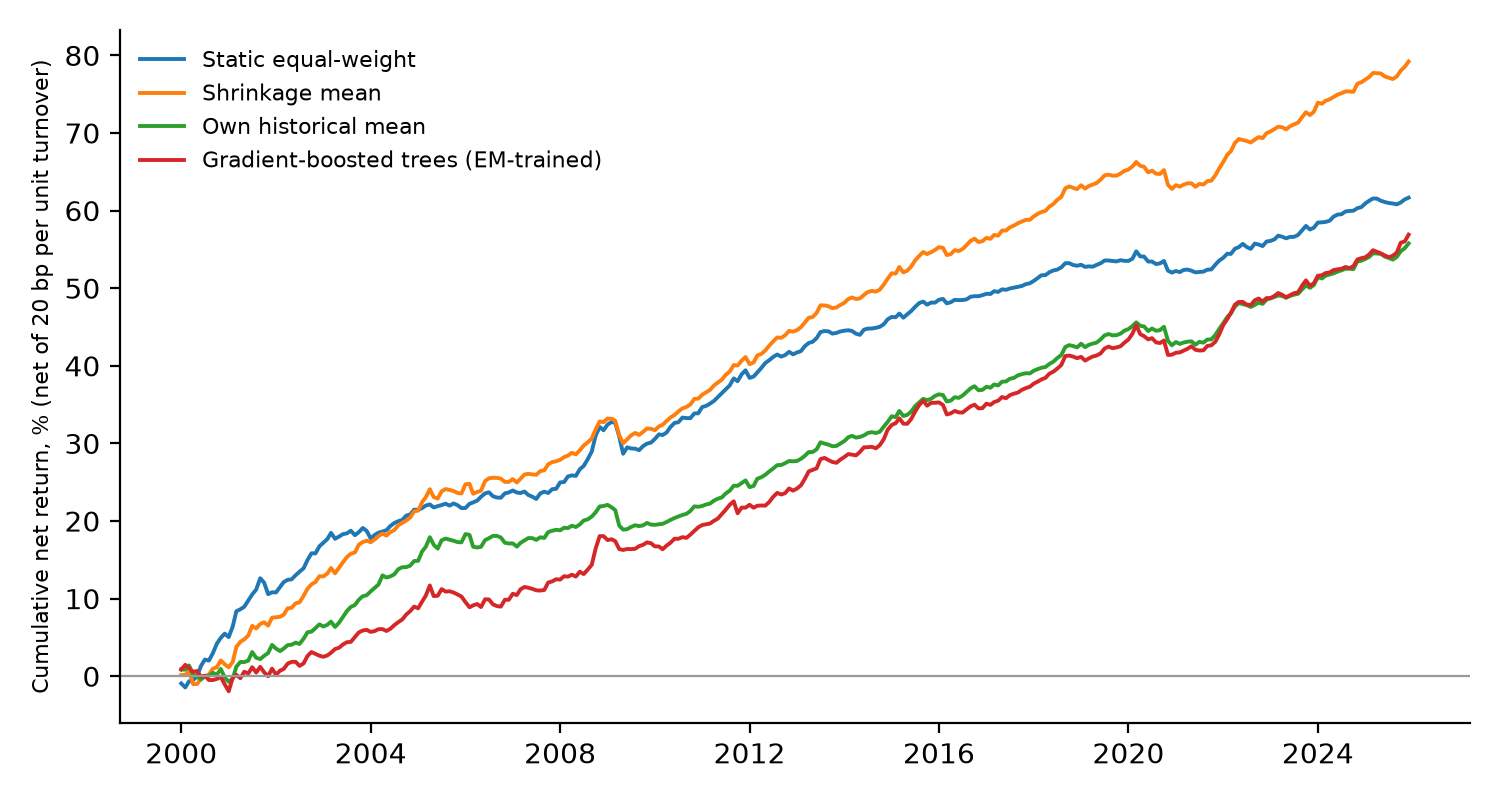
\includegraphics[width=0.9\linewidth]{figures/cumulative_net.png}
\caption{Cumulative net returns of emerging-market factor-timing portfolios, 2000--2025. Sum of monthly returns net of 20 basis points per unit of turnover, for the static equal-weight portfolio and the three strategies with the highest net Sharpe ratios.}
\label{fig:cum}
\end{figure}

\subsection{Robustness}
Table~\ref{tab:robust} varies the benchmark's prior weight $\kappa$, the start of the evaluation sample, the weighting of the factor portfolios, the market classification and the cost. The time-varying classification assigns each country-month the MSCI class then in force (Appendix~\ref{app:classification}): it moves Greece out of the emerging-market sample for 2001--2013, adds Argentina, Morocco, Pakistan and Russia during their emerging-market years, and admits Qatar, the United Arab Emirates, Saudi Arabia and Kuwait only after their upgrades. The neural network is run only in the baseline.

Three results are stable. In every row the shrinkage mean beats the own historical mean, by 0.97--1.37\% in $R^2_{OS}$, and the shrinkage-mean portfolio has the highest net Sharpe ratio. And the Clark--West statistics of the EM- and DM-trained trees stay above 2.8, with one exception: EM-trained trees on uncapped value-weighted factors (1.21).

Three results depend on the specification. First, the linear models' Clark--West statistics are sensitive to $\kappa$ and to factor weighting: 3.1--3.3 with $\kappa = 60$, but 0.8--1.5 with $\kappa = 240$ and 1.3--1.5 with uncapped value-weighted factors. A weaker prior leaves more of the noise in each country-factor mean in the benchmark, which the models can again correct by pooling --- the same mechanism that inflates tests against the own mean. The linear-model evidence of timing on value-weighted factors is therefore fragile.

Second, equal-weighted factors behave differently. Seven of the nine learned model-by-scope combinations beat the shrinkage mean, with $R^2_{OS}$ up to 0.17\% (pooled elastic net) and Clark--West statistics of 3.8--5.0, and every learned-model portfolio beats the static portfolio net of 20 basis points (2.28--3.08 against 2.01), though none beats the shrinkage-mean portfolio (3.90). Equal weighting gives more weight to small stocks, which are the most expensive to trade, and the cost charged per unit of turnover is the same for every weighting, so these Sharpe ratios are the least implementable in the table.

Third, the comparison of timing portfolios with the static portfolio depends on costs: at 10 basis points the EM-trained tree portfolio's net Sharpe ratio (1.60) exceeds the static portfolio's (1.49), though it stays below the shrinkage-mean portfolio's (1.95); at 40 basis points the learned-model portfolios fall to 0.05--0.59. Stronger shrinkage also improves the benchmark itself: its $R^2_{OS}$ against the own mean rises from 0.98\% at $\kappa = 60$ to 1.36\% at $\kappa = 240$, which suggests that emerging-market factor premia differ across countries less than their sample means do.

Not yet run: U.S. dollar, VIX and U.S. term-spread state variables for the developed-to-emerging channel, and size-dependent trading costs.

\begin{table}[!ht]
\centering\footnotesize
\caption{Robustness}
\label{tab:robust}
\begin{tabular}{lrrrrrrrrr}
\toprule
\multicolumn{10}{l}{\textit{Panel A: $R^2_{OS}$ (\%) and Clark--West $t$ against the shrinkage mean}} \\
\addlinespace
 & Shrink.\ vs.\ & \multicolumn{2}{c}{Elastic net, EM} & \multicolumn{2}{c}{Elastic net, DM} & \multicolumn{2}{c}{GBRT, EM} & \multicolumn{2}{c}{GBRT, DM} \\
\cmidrule(lr){3-4}\cmidrule(lr){5-6}\cmidrule(lr){7-8}\cmidrule(lr){9-10}
Specification & own mean & $R^2$ & $t$ & $R^2$ & $t$ & $R^2$ & $t$ & $R^2$ & $t$ \\
\midrule
Baseline & 1.203 & $-$0.046 & 1.56 & $-$0.174 & 2.08 & $-$0.212 & 3.66 & $-$0.233 & 3.79 \\
OOS from 2005 & 0.972 & $-$0.005 & 1.89 & $-$0.132 & 1.99 & 0.011 & 3.51 & $-$0.170 & 3.11 \\
$\kappa = 60$ & 0.976 & $-$0.004 & 3.13 & $-$0.129 & 3.08 & $-$0.195 & 4.48 & $-$0.176 & 4.46 \\
$\kappa = 240$ & 1.356 & $-$0.069 & 0.79 & $-$0.197 & 1.52 & $-$0.265 & 2.88 & $-$0.261 & 3.45 \\
Equal-weighted factors & 1.370 & 0.114 & 3.79 & 0.103 & 4.14 & $-$0.020 & 4.34 & $-$0.041 & 4.74 \\
Uncapped value-weighted & 1.194 & $-$0.054 & 1.28 & $-$0.129 & 1.37 & $-$0.294 & 1.21 & $-$0.247 & 3.14 \\
Time-varying classification & 1.229 & $-$0.047 & 1.84 & $-$0.183 & 2.02 & $-$0.240 & 3.66 & $-$0.318 & 3.28 \\
\bottomrule
\end{tabular}

\vspace{10pt}
\begin{tabular}{lrrrrrr}
\toprule
\multicolumn{7}{l}{\textit{Panel B: net Sharpe ratios of timing portfolios}} \\
\addlinespace
 & & Shrinkage & \multicolumn{2}{c}{Elastic net} & \multicolumn{2}{c}{GBRT} \\
\cmidrule(lr){4-5}\cmidrule(lr){6-7}
Specification & Static & mean & EM & DM & EM & DM \\
\midrule
Baseline & 1.48 & 1.91 & 1.11 & 0.74 & 1.26 & 1.13 \\
OOS from 2005 & 1.34 & 1.79 & 1.25 & 0.77 & 1.34 & 0.99 \\
$\kappa = 60$ & 1.48 & 1.73 & 1.00 & 0.70 & 1.15 & 1.09 \\
$\kappa = 240$ & 1.48 & 2.05 & 1.19 & 0.77 & 1.31 & 1.15 \\
Equal-weighted factors & 2.01 & 3.90 & 2.76 & 2.31 & 3.08 & 2.51 \\
Uncapped value-weighted & 1.45 & 1.80 & 1.03 & 0.74 & 1.10 & 1.06 \\
Time-varying classification & 1.56 & 1.97 & 1.19 & 0.83 & 1.43 & 1.05 \\
Cost 10 bp & 1.49 & 1.95 & 1.38 & 1.08 & 1.60 & 1.47 \\
Cost 40 bp & 1.45 & 1.81 & 0.58 & 0.05 & 0.59 & 0.43 \\
\bottomrule
\end{tabular}

\vspace{4pt}
\begin{minipage}{0.97\linewidth}\footnotesize
\textit{Notes:} Emerging-market test set. Baseline: $\kappa=120$, 20 bp per unit of turnover, out of sample 2000--2025. ``OOS from 2005'' keeps the baseline forecasts for target months from 2005, which equal those of a rerun starting in 2005 because models are refitted annually on an expanding window. $\kappa$ rows rerun the full pipeline, changing both the benchmark and the learned models' anchor. Factor-weighting rows rerun it on equal-weighted or uncapped value-weighted JKP factors. ``Time-varying classification'' assigns each country-month the MSCI class then in force (Appendix~\ref{app:classification}). Cost rows change only the charge per unit of timing turnover. ``Shrink.\ vs.\ own mean'' is the $R^2_{OS}$ of the shrinkage mean against the own historical mean. EM / DM = trained on emerging / developed markets only.
\end{minipage}
\end{table}


\section{Conclusion}
Emerging-market factor returns contain a small amount of predictable time variation. It is detectable out of sample, including by models trained only on developed markets, but in capped value-weighted factors it is too small relative to forecast noise and trading costs to be worth timing. In equal-weighted factors, which lean toward small stocks, it is larger, and timing portfolios beat a static factor portfolio net of a uniform 20-basis-point cost that likely understates the cost of trading those stocks. The larger and more robust gain is in estimating the unconditional premia themselves: pooling each factor's history across emerging markets beats the own historical mean with an $R^2_{OS}$ of 1.20\% and gives the best portfolio net of costs in every specification. The methodological point follows. In multi-country factor panels, out-of-sample tests against the own historical mean mostly measure that pooling gain, and a pooled benchmark should replace it.

Several extensions remain. Shrinking forecasts toward the benchmark with a factor estimated in real time could address the overstated amplitude documented in Table~\ref{tab:r2}; size-dependent trading costs would test whether the equal-weighted gains survive; and global state variables would help explain why developed-market history is informative.

\clearpage
\bibliography{references}

\clearpage
\appendix
\section{Validation on known-truth simulated panels}
\label{app:validation}

The pipeline is validated on simulated panels in which the predictable part of returns is known. For country $c$ and factor $f$,
\begin{equation}
r_{c,f,t+1} = \mu_{c,f} + x_{c,f,t} + e_{c,f,t+1}, \qquad
x_{c,f,t} = \sqrt{\rho}\, z_{f,t} + \sqrt{1-\rho}\, u_{c,f,t},
\label{eq:dgp}
\end{equation}
where $\mu_{c,f} \sim N(0.002, 0.003^2)$, $z$ and $u$ are independent AR(1) processes with persistence 0.95 and standard deviation $\sigma_x$, $\rho = 0.6$ is the share of the predictable component common to all countries, and $e \sim N(0, 0.03^2)$. Setting $\sigma_x = 0$ removes all predictability.

\paragraph{Why the own mean over-rejects.} The Clark--West term $2(r-b)(\hat r - b)$ has positive expectation whenever the forecast corrects the benchmark's own estimation error. With heterogeneous $\mu_{c,f}$ and short histories, $\bar r_{i,t}$ is noisy, and a pooled model learns to shrink it --- a genuine improvement in estimating $\mu_{c,f}$ that the test attributes to timing. Anchoring on the shrinkage mean~\eqref{eq:shrink} removes most of that error before the model is fitted.

\begin{table}[!ht]
\centering
\caption{Size and power of the Clark--West test on known-truth synthetic panels}
\label{tab:sizepower}
\begin{tabular}{lrrrrr}
\toprule
 & & \multicolumn{2}{c}{vs.\ own historical mean} & \multicolumn{2}{c}{vs.\ shrinkage mean} \\
\cmidrule(lr){3-4}\cmidrule(lr){5-6}
Signal s.d. & Draws & Mean $R^2_{OS}$ (\%) & Reject (\%) & Mean $R^2_{OS}$ (\%) & Reject (\%) \\
\midrule
0 (null) & 40 & 0.058 & 87.5 & -0.055 & 5.0 \\
0.004 & 40 & 0.264 & 97.5 & 0.133 & 92.5 \\
0.008 & 40 & 1.773 & 100.0 & 1.599 & 100.0 \\
\bottomrule
\end{tabular}

\vspace{4pt}
\begin{minipage}{0.92\linewidth}\footnotesize
\textit{Notes:} Simulated data, not a finding. Each draw is a panel of 6 developed and 6 emerging
markets, 12 factors and 300 months generated by equation~\eqref{eq:dgp}; the pooled OLS model is
evaluated out of sample from 2005. ``Reject'' is the share of draws with a one-sided Clark--West
$t$-statistic above 1.645. The first row has no predictability, so its rejection rate is the
empirical size of a nominal 5\% test.
\end{minipage}
\end{table}


Table~\ref{tab:sizepower} reports 40 draws at each signal level. Against the own historical mean, the test rejects in 87.5\% of null draws. Against the shrinkage mean, the rejection rate under the null is 5.0\%, equal to the nominal size, and power is 92.5\% and 100\% at the two signal levels. In separate draws with predictability shared across countries ($\rho = 0.6$), models trained only on developed markets also recover it in emerging markets, so the transfer test can detect transfer when it exists.

\clearpage
\section{Time-varying market classification}
\label{app:classification}

The baseline classifies markets by the current MSCI classification. The robustness check in Table~\ref{tab:robust} instead uses the class in force in each month. Table~\ref{tab:classification} lists the reclassifications within the sample that involve developed or emerging status; each takes effect from the first full month after MSCI implemented it. A market's training and test assignment use its class in month $t$. The pooled regional mean for region $g$ averages every past country-month that belonged to $g$ when it was observed, and the developed-market predictor averages the markets classified as developed at $t$. First inclusion in the MSCI indexes and partial-inclusion steps are not modelled.

\begin{table}[!ht]
\centering\footnotesize\setlength{\tabcolsep}{4pt}
\caption{MSCI reclassifications used for the time-varying classification}
\label{tab:classification}
\begin{tabular}{llll}
\toprule
Market & In force from & New class & MSCI event \\
\midrule
Portugal & 1997-12 & Developed & Emerging $\to$ Developed, Nov 1997 \\
Greece & 2001-06 & Developed & Emerging $\to$ Developed, May 2001 \\
Venezuela & 2006-06 & Frontier/standalone & Emerging $\to$ Standalone, May 2006 \\
Jordan & 2008-12 & Frontier/standalone & Emerging $\to$ Frontier, Nov 2008 \\
Pakistan & 2009-01 & Frontier/standalone & Emerging $\to$ Standalone, close of 31 Dec 2008 \\
Argentina & 2009-06 & Frontier/standalone & Emerging $\to$ Frontier, May 2009 \\
Israel & 2010-06 & Developed & Emerging $\to$ Developed, May 2010 \\
Greece & 2013-12 & Emerging & Developed $\to$ Emerging, Nov 2013 \\
Morocco & 2013-12 & Frontier/standalone & Emerging $\to$ Frontier, Nov 2013 \\
United Arab Emirates & 2014-06 & Emerging & Frontier $\to$ Emerging, May 2014 \\
Qatar & 2014-06 & Emerging & Frontier $\to$ Emerging, May 2014 \\
Pakistan & 2017-06 & Emerging & Frontier $\to$ Emerging, effective 1 Jun 2017 \\
Argentina & 2019-06 & Emerging & Frontier $\to$ Emerging, May 2019 \\
Saudi Arabia & 2019-06 & Emerging & Standalone $\to$ Emerging, May 2019 (step 1 of 2) \\
Kuwait & 2020-12 & Emerging & Frontier $\to$ Emerging, close of 30 Nov 2020 \\
Argentina & 2021-12 & Frontier/standalone & Emerging $\to$ Standalone, Nov 2021 \\
Pakistan & 2021-12 & Frontier/standalone & Emerging $\to$ Frontier, Nov 2021 \\
Russia & 2022-04 & Frontier/standalone & Emerging $\to$ Standalone, close of 9 Mar 2022 \\
\bottomrule
\end{tabular}

\vspace{4pt}
\begin{minipage}{0.95\linewidth}\footnotesize
\textit{Notes:} Each market takes the new class from the first full month after MSCI implemented the change; before its first event a market has its prior class, and markets without events keep their current class. First inclusion in the MSCI indexes and partial-inclusion steps are not modelled. Sources: MSCI's list of market reclassifications and MSCI announcements, cited in \texttt{config/market\_history.yaml}.
\end{minipage}
\end{table}


\end{document}
